\documentclass[sigplan,10pt]{acmart}
\usepackage[utf8]{inputenc}
\usepackage{todonotes}

\setcopyright{rightsretained}
\copyrightyear{2020}
\acmYear{2020}
\acmDOI{}
\acmConference[]{}{}{}
\acmBooktitle{}
\acmPrice{}
\acmISBN{}

\hyphenation{Web-RTC}

\begin{document}
\title{PushPin: Towards Production-Quality  Peer-to-Peer Collaboration}

\author{Peter van Hardenberg}
\email{pvh@inkandswitch.com}
\affiliation{%
  \institution{Ink \& Switch, LLC}
  \city{San Francisco}
  \state{CA}
  \postcode{}
  \country{USA}
}

\author{Martin Kleppmann}
\email{mk428@cl.cam.ac.uk}
\orcid{0000-0001-7252-6958}
\affiliation{%
  \institution{University of Cambridge}
  \streetaddress{15 JJ Thomson Avenue}
  \city{Cambridge}
  \state{}
  \postcode{CB3 0FD}
  \country{United Kingdom}
}

\begin{abstract}
Fully peer-to-peer application software promises many benefits over cloud software, in particular, being able to function indefinitely without requiring servers.
Research on distributed consistency mechanisms such as CRDTs has laid the foundation for P2P data synchronisation and collaboration.
In this paper we report on our experience in taking these technologies beyond research prototypes, and working towards commercial-grade P2P collaboration software.
We identify approaches that work well in our experience, such as the functional reactive programming paradigm, and highlight areas in need of further research, such as the reliability of NAT traversal and usability challenges.
\end{abstract}

\begin{CCSXML}
<ccs2012>
    <concept>
        <concept_id>10003033.10003039.10003051.10003052</concept_id>
        <concept_desc>Networks~Peer-to-peer protocols</concept_desc>
        <concept_significance>500</concept_significance>
    </concept>
    <concept>
        <concept_id>10011007.10010940.10010971.10010972.10010540</concept_id>
        <concept_desc>Software and its engineering~Peer-to-peer architectures</concept_desc>
        <concept_significance>500</concept_significance>
    </concept>
    <concept>
        <concept_id>10003120.10003130.10003233</concept_id>
        <concept_desc>Human-centered computing~Collaborative and social computing systems and tools</concept_desc>
        <concept_significance>500</concept_significance>
    </concept>
    <concept>
        <concept_id>10011007.10010940.10010992.10010993.10010961</concept_id>
        <concept_desc>Software and its engineering~Synchronization</concept_desc>
        <concept_significance>300</concept_significance>
    </concept>
</ccs2012>
\end{CCSXML}

\ccsdesc[500]{Networks~Peer-to-peer protocols}
\ccsdesc[500]{Software and its engineering~Peer-to-peer architectures}
\ccsdesc[500]{Human-centered computing~Collaborative and social computing systems and tools}
\ccsdesc[300]{Software and its engineering~Synchronization}

\keywords{real-time collaboration, CRDTs, peer-to-peer protocols, distributed programming, usability}

\maketitle

\section{Introduction}

In the past, software used to run on one computer and store its data on the local disk.
Now, increasingly, we expect our software and data to be available on multiple devices, with synchronisation across devices belonging to the same user (e.g.\ laptop, smartphone, tablet), and also allowing real-time collaboration between multiple users.

The standard way of implementing such multi-user, multi-device software today is to rely on cloud services that store the authoritative copy of the users' data, and which can be accessed through thin clients such as web browsers and mobile apps.
However, reliance on the cloud comes with problems: services require ongoing maintenance by expensive 24/7 operations teams, and they cease to exist when the organisation backing them terminates their funding.
If a cloud service shuts down, users lose access to all data stored in that service, unless some migration path to an alternative service is provided.
Moreover, cloud-centric software often does not work well offline, and can be slow as the client waits for round-trips to the server in order to load or store data there.

Peer-to-peer application software promises to overcome these problems.
In principle, a P2P system should be able to function indefinitely, without depending on someone paying the server bills to keep a cloud service running.
Storing an authoritative copy of data on the users' devices enables offline work and stronger data ownership~\cite{LocalFirst}, and synchronising updates through a P2P network should allow the same kind of real-time collaboration that we know from cloud software.

While various research prototypes of P2P collaboration software have been developed, we are yet to see any mainstream applications using this approach.
The PushPin project is investigating if and how we can develop commercial-quality collaboration software with minimal reliance on servers.
Our goal is not to create new algorithms or protocols, but rather to evaluate existing technologies by developing an example P2P application with a mindset of industrial software development best practices.
We approach this project with broad interests in exploring programming models, P2P data distribution, reliability, and usability.

In summary, our findings are:
\begin{itemize}
    \item TODO fill in these bullet points with some punchy statements when we've written the rest of the article
    \item \dots
\end{itemize}

% The prize for delivering a truly peer-to-peer application development system is great.
% centralised cloud-based software has created the expectation of universal access to both canonical versions of software and to users' data from any internet-connected computer at any moment, with full collaborative functionality built in.

%To this end, we must reconsider our relationship with vast centralised databases and explore new methodologies for building software.

% document CRDTs
% functional reactive programming
% browser rendering
% "document oriented programming"

\section{Design Principles}\label{sec:principles}

Before going into the details of the implementation of PushPin we outline the principles we applied to its design and development.

\subsection{Local-first software}

While we want users' data to be accessible on multiple devices, the authoritative copies of this data should reside on the users' local computers, not in the cloud.
If servers are used, these replicas should be considered secondary copies that exist only to facilitate data synchronisation and backup, but they should not be considered authoritative.
In previous work we have coined the term \emph{local-first software} to describe software that adheres to this principle~\cite{LocalFirst}.

With a local-first approach, the software continues working fully if the user's computer is disconnected from the Internet: cross-device synchronisation happens in the background when a network connection is available.
Even if all servers are shut down, the copy of the data on the local disk remains fully functional and under the user's control.
The user can manage this data like any other local files, e.g.\ copying it, backing it up, or converting it into another format.

\subsection{Minimal dependence on servers}

We want the software to continue working indefinitely, without incurring ongoing costs for operating servers.
Thus, in addition to local data storage on each device, the cross-device data synchronisation mechanism should also depend on servers to the least degree possible.

In some environments it is possible to operate entirely without servers, while in other cases a small amount of centralised infrastructure seems to be inevitable with current technologies.
We discuss these issues in detail in Section~\ref{sec:networking}.

\subsection{Conflict-free data synchronisation}

The combination of using local on-device storage, support for offline editing, and synchronisation without servers implies that our application is \emph{intrinsically distributed}.
Each device serves as a replica, and it would not make sense to enforce any kind of single system image semantics across replicas, since that would imply that a device must wait for synchronous coordination with other devices whenever any data is changed.
We cannot rely on consensus algorithms, which must wait for communication with a quorum of replicas.

Rather, we have to accept that each device has its own local view onto the shared data, and that those views may diverge as users update their data.
As devices exchange updates, they converge again by merging their states.
We do this using conflict-free replicated data types (CRDTs)~\cite{Shapiro:2011un}.

\subsection{Mainstream, as far as possible}

In order to explore the \emph{user experience} implications of a peer-to-peer architecture, we wanted to develop not just a rough research prototype, but polished end-user software that is on par with commercial applications available today, with a thoughtful graphical and interaction design.
We also wanted to explore the \emph{developer experience} of peer-to-peer software, to understand how this architecture could become accessible to mainstream software engineers.
Thus, we wanted to base our work on mainstream languages and platforms as far as possible.

\begin{figure*}
    \centering
    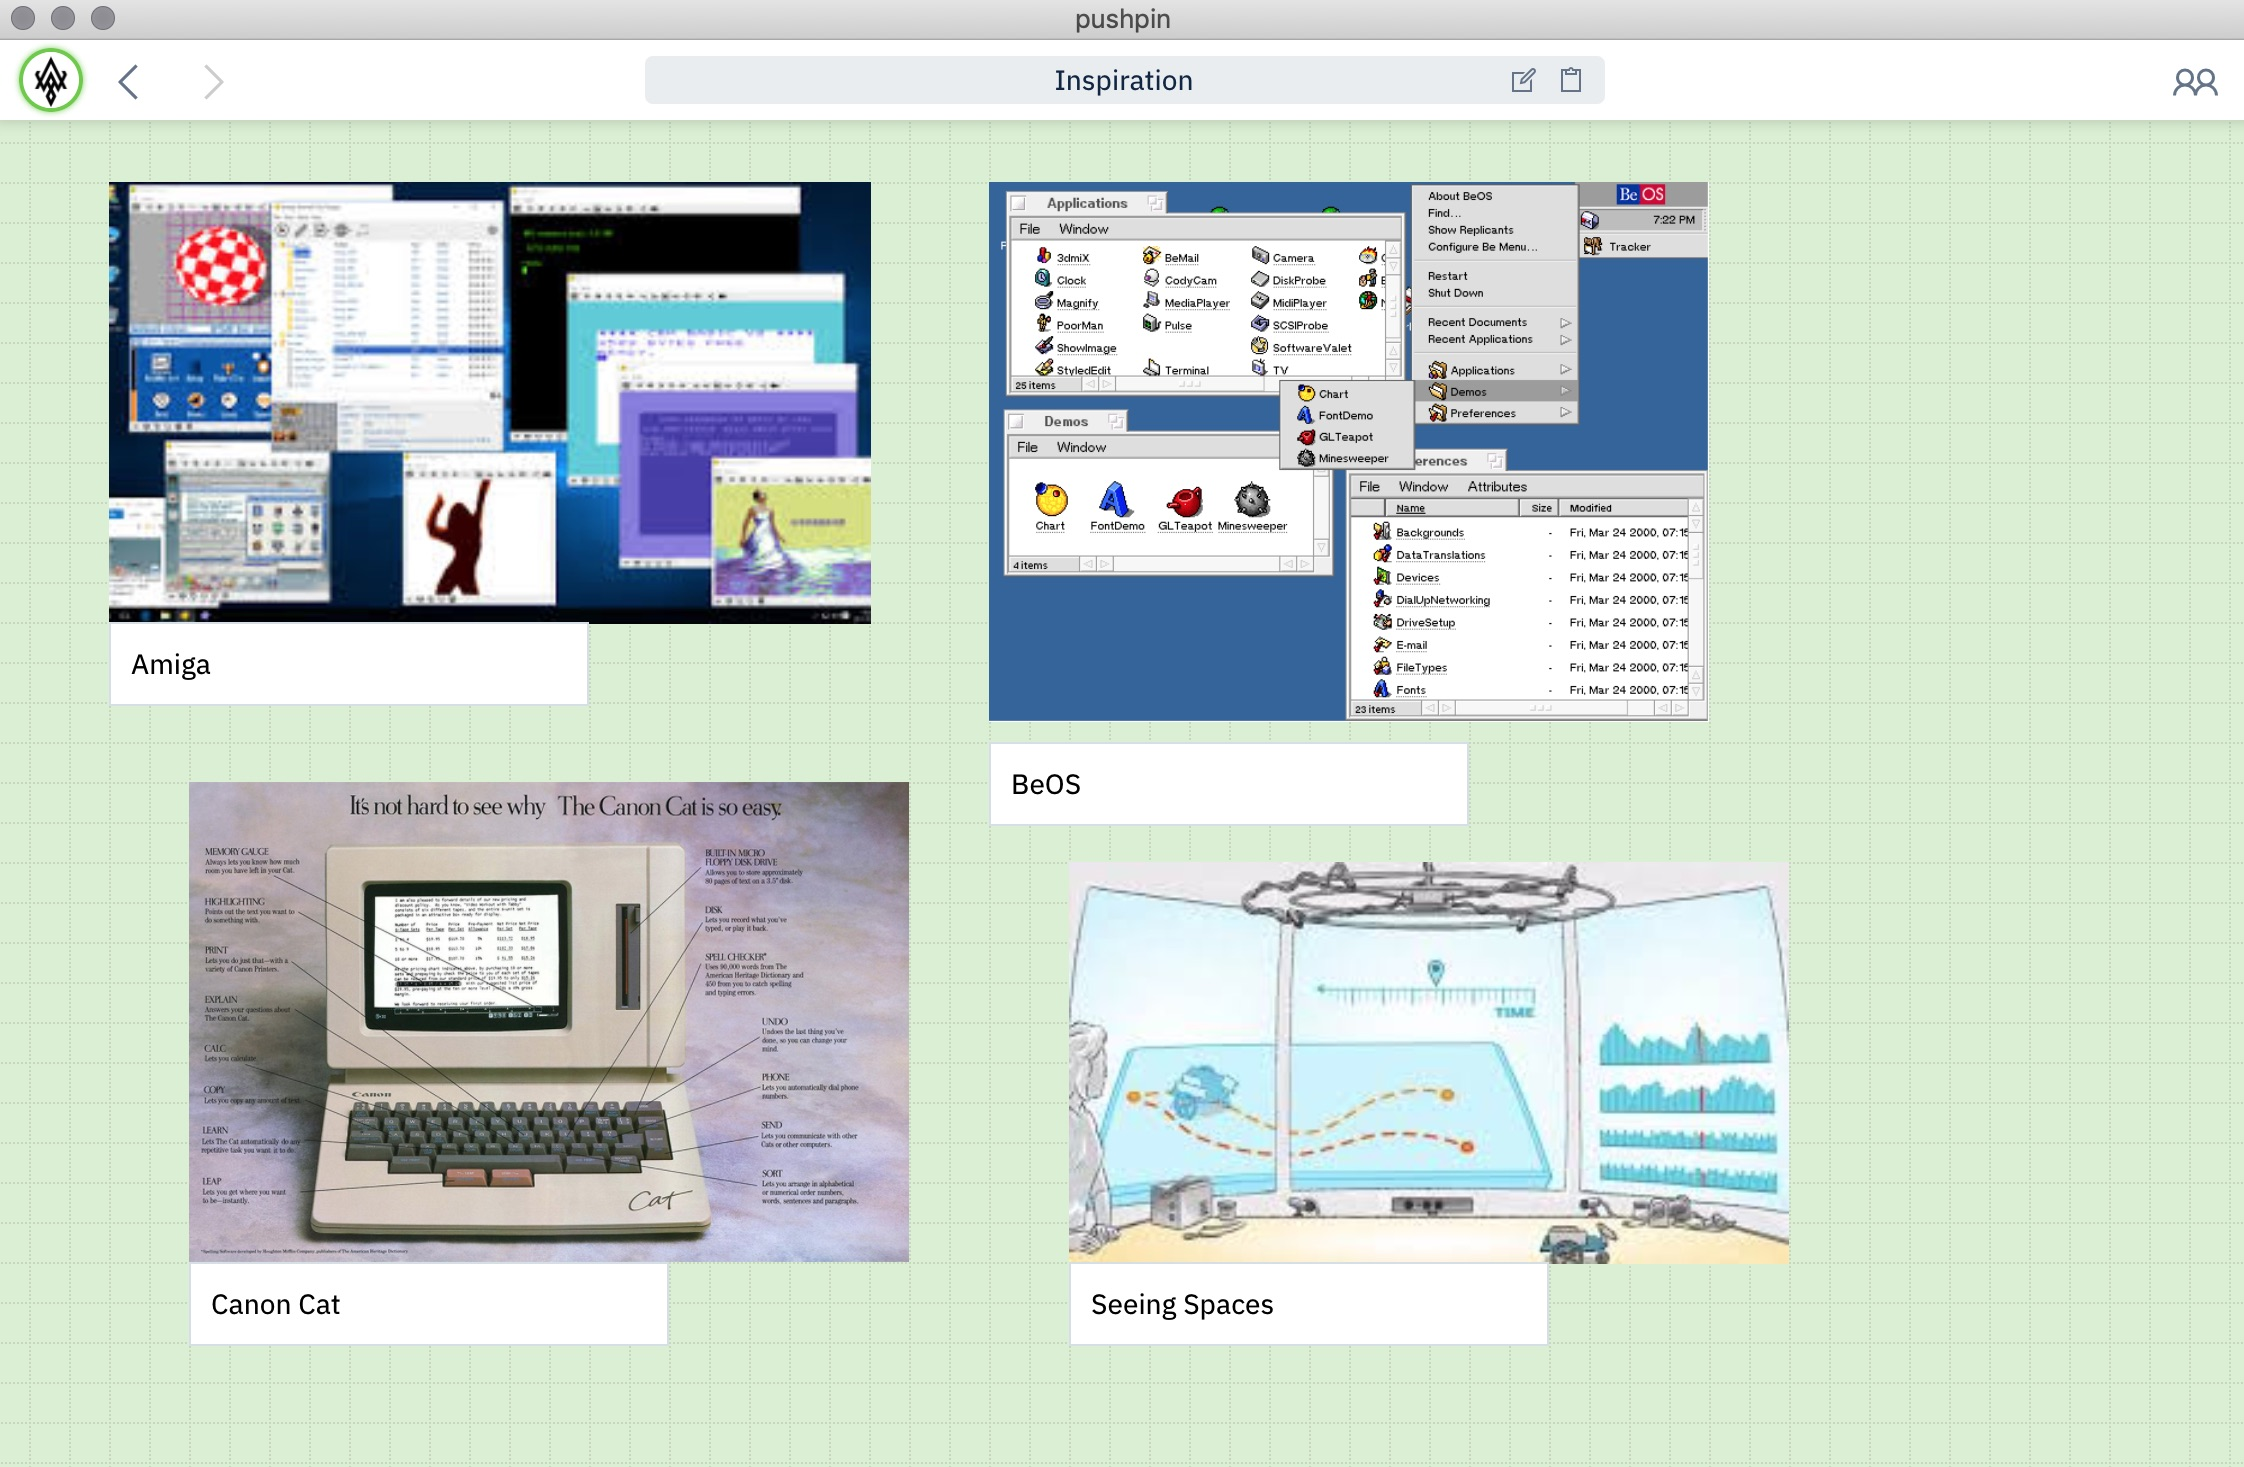
\includegraphics[width=0.7\textwidth]{pushpin.jpg}
    \caption{Screenshot of PushPin. The main user interface consists of cards of various types (text, image, PDF, \dots) that can be freely arranged on a 2D ``board''. Boards can be nested within other boards. The toolbar at the top provides navigation between boards and sharing settings.}
    \label{fig:pushpin}
\end{figure*}

\section{PushPin: A Collaborative Corkboard}\label{sec:pushpin}

The PushPin software~\cite{PushPinSource}, shown in Figure~\ref{fig:pushpin}, allows users to collect media of various types (including text, web pages, images, and PDF files), to archive and organise it.
Media files are visually represented as \emph{cards} on an infinite two-dimensional \emph{board}, where they can be resized and positioned arbitrarily.
One board may be nested within another board, enabling hierarchical organisation and navigation.
This board metaphor is known from other note-taking software such as Miro~\cite{Miro} and Milanote~\cite{Milanote}.

We have built PushPin upon the principles articulated in Section~\ref{sec:principles}.
In this section we go into the details of our technology choices implementing PushPin, and we report on lessons we learnt in Section~\ref{sec:lessons}.

\subsection{Building desktop software with Electron}

In recent years there has been considerable innovation in web application technologies, including in web browsers (new features of HTML and CSS), languages (e.g.\ TypeScript), user interface libraries (especially React~\cite{React}), and JavaScript modules for a wide variety of tasks (e.g.\ PDF rendering~\cite{PDFjs}).
In order to take advantage of this lively ecosystem, we decided to implement PushPin using web technologies.

However, web applications running in a browser tab have constraints that make them unsuitable for local-first/P2P use.
In particular, although web apps can write data to disk using APIs such as localStorage and IndexedDB, this data tends not to be very durable: it is silently deleted when a user chooses to clear cookies in their browser~\cite{LocalStorageCleared}.
(Maybe the clue is in the name: they are called ``browsers'', not ``keepers''.)

We avoid these limitations by building on Electron~\cite{Electron}, which takes a JavaScript web app, runs it in a Chromium-based browser window, and allows the result to be packaged as a downloadable and locally installed executable.
Electron makes Node.js APIs available to application code, including full access to the local filesystem, and socket APIs allowing arbitrary TCP and UDP networking.
(In contrast, in a browser tab, network communication is constrained for security reasons by the same-origin policy~\cite{SameOrigin}.)
Electron apps are portable across Windows, Linux, and macOS.

\subsection{Persistent State and Ephemeral State}

Every user interaction results in a state change within the application.
Broadly speaking, there are two types of state:
\begin{description}
\item[Persistent state] is saved to disk and replicated to other devices.
For example, the contents of every board and every card are represented as a JSON \emph{document}.
We use the Automerge CRDT library~\cite{Automerge,Automerge:2018} to represent all persistent documents, to replicate them, and to automatically merge any updates made concurrently on different devices.
\item[Ephemeral state] exists only in-memory in the locally running application, and is not replicated.
Ephemeral state includes the currently viewed board (TODO is this true?), the scroll position within a board view, or the unsaved draft contents of text boxes.
\end{description}

% TODO include an example JSON representation of a card?

% introduce URLs explicitly, explain how one document references another

Our earliest prototypes assumed users would have only a single "document" open at a time, and that these documents would be shared by their URLs. We also made no allowances for non-shared state. This model was very limiting, and over time we found we needed a number of additional concepts.

We added a messaging system to allow users to broadcast parts of this local state to their peers. We use this to communicate data which is valuable only in the moment and not worthy of recording, such as another users' current selection, or cursor position in a text field.

\subsection{Functional Reactive Programming}
The first motivating insight is that functional reactive programming~\cite{Czaplicki:2013ig} is a helpful abstraction. Functional reactive programming works by creating a single, functional loop where a program state is deterministically transformed into a user interface, and where all interactions emitting from the user interface pass through a single function (known as a reducer) which produce the next state.

In the simplest case, we tie the program state to an operational CRDT (automerge), and record all changes to that program state into a per-client append-only log which we can broadcast to our other peers. Visibility vectors preserve causality of changes, and for further details of how this process works, please see <some reference here>.

\begin{figure}
    \centering
    % diagram depicting FRP + CRDTs here
    %\includegraphics{}
    \caption{Caption}
    \label{fig:my_label}
\end{figure}

\subsection{Composite Views}

As we approached more sophisticated usage, we came across a simple idea that enabled us to preserve our abstraction while pursuing much more elaborate software. By allowing a pairing of a shareable CRDT document with an FRP renderer to be nested inside another such construct we can build up complex networks of documents each with their own collaborators.

For example, we can define a "container" which renders a list of documents stored as a CRDT of document URLs, and a user might synchronise the full list across all their own devices, but only share some of them with their other collaborators.

% i think this is now covered above but left this here for reference
\begin{comment}
    how to rationalize all this?
    \begin{itemize}
	    \item FRP, for its easily reasoned-about loop: 
	    \begin{itemize}
			 \item transform a document functionally into an application view
			 \item create events in the application that trigger state updates
			 \item record \& broadcast state updates to peers
		\end{itemize}
	    \item many nested \& linked documents, each with their own render function
	    \begin{itemize}
		    \item a text note, a chat window, a user profile, a canvas
		\end{itemize}
	    \item store all local changes in append-only logs, distribute those logs to other interested peers
	    \item use cryptographic functions to produce self-validating data
	\end{itemize}
\end{comment}

% Many P2P protocols require sending and receiving arbitrary UDP packets.
% However, web browsers restrict network communication for security reasons, in particular through the \emph{same-origin policy}~\cite{SameOrigin}, making it impossible to implement such protocols in JavaScript alone.
% An exception is WebRTC, a P2P protocol that is built into web browsers.

% Designed to collect all the information you need and synchronise it across all your computers. PushPin supports taking notes, and can archive web content, images, PDFs, audio, video, and any other files you might want to hang out. It can synchronise across all your devices, and doesn't require any infrastructure to operate.


\subsection{Document-oriented Programming}
\begin{itemize}
    \item crdts
    \item frp
    \item peer-to-peer data distribution
\end{itemize}


\section{Peer-to-peer Networking for Collaboration}\label{sec:networking}

Every networked application relies on three core facilities provided by the networking stack: discovering the network address to connect to, establishing a connection, and securing the confidentiality and integrity of the data transfer.

In a traditional web application, discovery is provided by DNS, connection by TCP, and security by SSL/TLS.
However, these technologies are not a good fit with our goal of minimising centralised infrastructure and ongoing cost:
\begin{itemize}
    \item DNS requires paying ongoing registration fees for domain names, and it requires running DNS servers.
    \item TCP requires the server to have a publicly routable IP address; it cannot connect directly to most end-user devices as they are behind NAT (see Section~\ref{sec:nat-traversal}).
    \item SSL/TLS certificates are tied to domain names, which incur registration fees.
\end{itemize}

The peer-to-peer technologies we explored in PushPin attempt to overcome the need for centralised infrastructure.

\subsection{Existing Peer-to-Peer Technologies}

We considered several P2P networking stacks for PushPin:
\begin{description}
\item[WebRTC] is a peer-to-peer protocol built into modern web browsers.
It is primarily designed for audio and video calls, but it can also carry application data.
WebRTC does not provide a peer discovery mechanism; typically, applications rely on a server to help peers discover each others' IP addresses (this process is called \emph{signaling}).
\item[BitTorrent] is widely used for file sharing.
It provides a distributed hash table (DHT) for peer discovery, and uses the uTP protocol to establish connections between peers.
However, it is designed for static files, and is not suitable for data that is constantly changing, like in collaboration software.
\item[IPFS] aims to provide decentralised storage through a networking stack called \emph{libp2p}.
Like BitTorrent, it is mostly focused on replicating static files; it provides limited support for changing data through its IPNS and PubSub modules, but these features are immature at the time of writing.
\item[Dat] is a peer-to-peer data sharing platform.
For peer discovery it uses a centralised DNS service hosted by a nonprofit foundation (a distributed hash table is under development), and it uses BitTorrent's uTP protocol to establish connections.
\end{description}

PushPin builds upon the \emph{hypercore} protocol and implementation from the Dat project~\cite{HowDatWorks}, since its focus on replicating mutable data makes it the best fit for our needs.

A hypercore is an append-only log that is authenticated with a public key; only the owner of the corresponding private key can modify the log, but many peers can store replicas of the log.
We map each PushPin document to a set of hypercores, with one hypercore per device that has edited the document.

\subsection{Peer Discovery}

The Dat protocol allows the replicas of a hypercore to be discovered based on a hash of its public key~\cite{HowDatWorks}.
We encode this public key in the form of a URL; thus, the URL is a stable identifier for the document, even as its content changes.
Knowledge of the URL allows a peer to obtain a copy of the document, via the peer discovery mechanism.
We allow one document to reference another by including the referenced document's URL in another document.

When peers are on the same LAN (wired or wireless network), they attempt to discover one another using mDNS, a variation on DNS that broadcasts DNS-like service advertisements or discovery requests to a well known multicast IP address.
If successful, the peers can connect directly via TCP and begin exchanging data.
This mode of discovery is appealing since it depends only on the local network: communication between peers does not flow via the Internet, and it does not depend on any centralised infrastructure.

When peers are not on the same LAN, the Dat protocol uses a centralised DNS server for peer discovery.
This approach is not fully peer-to-peer, but at present this seems to be a necessary compromise to make.

\subsection{NAT Traversal}\label{sec:nat-traversal}

% citations needed

Due to a shortage of IPv4 addresses, most personal computing devices do not have a globally reachable IP address, but rather a local address in a reserved space (e.g.\ 192.168.x.x or 10.x.x.x).
When such a device wishes to establish a connection to another, the local router records the destination of outbound traffic and routes responses back to the originating local client.
This process is called Network Address Translation (NAT).

A device behind NAT can only make outbound connections, but it cannot receive inbound TCP connections.
An exception: in home environments, where the user has control over their own router, the UPnP standard allows clients to reserve particular ports on the router as the destination for inbound connections.
However, mobile devices often use networks on which UPnP is not available, such as a coffee shop WiFi, a corporate office network, or a cellular data network.

In these cases, the most viable solution is known as ``hole punching'' or NAT traversal \cite{NatTraversal}.
This process requires the temporary intervention of a third host to introduce the two peers, and both peers sending UDP packets to each other, allowing a connection to be established.
NAT traversal is performed by BitTorrent's uTP protocol, and by the STUN protocol in WebRTC.

However, there are situations in which neither the LAN discovery approach nor NAT traversal works.
For example, some coffee-shop WiFi and some corporate networks are set up in a ``guest network'' mode, which prevents all local connections between devices on the network (intended as a security measure to prevent inadvertent sharing of data on the network).
Without local traffic, we attempt to fall back on NAT traversal; however, this approach also fails, since many routers in their default configuration refuse to create NAT traversing routes that originate and terminate within the same network.

In this case, establishing a direct connection between the peers seems to be impossible, and the only remaining option is to use a TURN server to proxy the communications between the peers.
In the case of PushPin, users can either run their own publicly addressable network hosts or take advantage of a TURN server provided by the community.

\subsection{Cloud Peers}

\todo[inline]{Martin is working from here onwards}

These ``cloud peers'' can perform not only the valuable service of providing indirect connections but given some storage space can also provide persistent network availability for data which would otherwise fall offline with the closing of every laptop lid.   

\subsection{Trust, but Verify}

Earlier we noted that traditional client-server protocols operate by providing cryptographic signatures proving posession of host authenticity. In an environment consisting of transient hosts we choose not to authenticate hosts but rather data itself. 

The most common approach to self-validating data is content addressable hashing, and used by BitTorrent. With content addressable hashing, the data is not requested by an arbitrary name or URL, but rather by a hash of its contents. (In fact, BitTorrent uses Merkle trees \cite{MerkleTrees} to allow efficient incremental validation of data during its download.) Short of compromising the hash function used to describe the data, it is impossible to spoof its contents. Unfortunately, changing even a single byte of data causes the hash to change. This makes content hashing unsuitable for real-time collaboration, as it is difficult to name a document that evolves over time.

\subsection{Stable Names}

Instead of naming a document by its contents, PushPin adopts a technique inherited again from the Dat Project \cite{DatProject} which is to create an log of messages, each signed (as with an SSL certificate) by an unpublished private key, but addressable by its public key. Because each new message includes both a signature from the private key and the signature of the preceding message, it is trivial to ensure integrity of the chain of messages, and messages can be downloaded from anyone.

These stable names are important for collaboration, because users often want to be able to share documents over time, as in the case of an essay as it is being written, or a PushPin board as cards are added to it, and to be able to link that content. If the names for content were unable to evolve, a single change to a document would require every document that referred to it to be republished with a new URL, which would require those documents' linkers to be republished and so on, ad infinitum. 

\subsection{Discovery in the Dark Forest}

We have, thus far, mostly ignored the subject of how one can identify which hosts possess the data a client wishes to request. We have established that with PushPin, as with many other peer-to-peer systems, documents provide their own validation tied to their specially chosen names. These names then, are in security terms a capability, which enable anyone who holds that key to access the contents of the document. Given the importance of these keys, how can we discover which other clients hold the keys without revealing them?

As noted above, the first step is to discuss not the key itself, but a cryptographic hash of the key. By hashing the key in a well-defined manner, any clients who know the underlying secret can agree on a public value to discuss. Without the ability to reverse the hashing function an observer might observe that clients are discussing a topic but cannot infer the key passively. (Once clients connect, both peers must provide a new, second cryptographic proof that they hold the underlying secret in order to outfox an attacker hoping to spoof their way in.)

Once we have this new, safe-to-discuss key, we can advertise it. On a local network, we can broadcast it over mDNS as describe above. Over the internet, we can use signalling servers as with WebRTC, or else we can post the keys into distributed hash tables as with BitTorrent where other peers can discover us and establish connections. (It should be noted that in practice today, the BitTorrent DHT has proven itself operationally resilient but other implementations such as IPFS have struggled to remain useful during flooding attacks.)

The simple, naive solution then, would be to broadcast all the hashes of every piece of data each client holds, and every hash it requests. This approach, used by the Dat Project \cite{DatProject} is suitable when the number of keys is small, but breaks down rapidly as collections expand. As we will see later, PushPin generates many hundreds or thousands of keys in its operation, and in our testing we found we fairly reliably crash the consumer WiFi routers found in short-term rentals with even as few as a half-dozen researchers sharing their collections.

% TODO: diagram of append-only logs, discovery keys, maybe broadcasting?

The Secure Scuttlebutt~\cite{Tarr:2019ba} project avoids this problem by placing all of a user's activity into a single log, which it then merges with all of that user's peers and their peers out for several degrees of social connection. This trades one problem for another! By merging all of a user's data (and their peers' data) into one feed, there is no way to selectively synchronise that user. A peer either downloads all, or none. 

Fortunately, we have observed that collaborators tend to collaborate on a variety of documents. The most likely place to discover a new document of interest is within the corpus of a peer you have already connected to. We can radically reduce the amount of discovery network traffic by doing normal queries not against a full, global DHT but against the repositories of peers we have already been introduced to. Perhaps these peers could also forward queries on our behalf, recreating a DHT-like network. This is an area for future work.

Finally, in closing for this section, it is worth noting that most current discovery solutions have large side-channel problems. Current implementations broadcast sufficient data that an attacker could passively join to the network, listen for discovery traffic and identify a user's device by the pattern of discovery keys it shares. The attacker need not know the contents of those keys, simply that the same hosts appear to appear and publish them over time. With this information, the attacker could track their target through physical space by monitoring their IP address over time. This is the dark forest from the section title. An attacker can lurk, passively, until a target compromises itself in important ways with no recourse whatsoever. There are a number of defences that could reduce these threat vectors (automatic rotation of discovery keys, or some form of lively proof exchange through a third party prior to exposing IP addresses) but this remains an area of active concern and research.

\subsection{Networking Conclusions}

By creating documents out of trustworthy append-only logs with stable names, we enable links and stably-named collaborative documents. A variety of state-of-the-art networking strategies overcomes the limitations of commonly available NAT routers in the field. Unfortunately, these techniques are not reliable enough to eliminate all traffic proxy requirements, and so we employ optional, but helpful network-persistent peers which act as relay points and data caches to improve reliability. (Importantly, they are not a central resource but can be run by any motivated network participant.) Last, we discuss some of our early work in improving discovery strategies for scalability without sacrificing specificity and some of the problems with current distributed hash table implementations today.

\section{Lessons from Implementing PushPin}\label{sec:lessons}

%Challenges of Developing an Intrinsically Distributed System

Peer-to-peer systems have a number of unique challenges versus centralised systems, including:

\begin{itemize}
	\item no single source of truth, no single authority

	Without a centralised server hosting an authoritative copy, every copy of the data becomes, in some sense, authoritative. This implies that we must have some kind of robust merging strategy at the core of our design.
	\item devices get out of sync

    Because we insist that each device is always able to make progress without communication with other nodes, it is vitally important to both do our best to synchronise our various devices, but also to communicate synchronisation state. What were the last changes received from our laptop? Did the changes we made locally get uploaded to a server before the network connection was lost?  

    \item connectivity is non-boolean

    With a centralised system a user is either offline or online. The central node routes all data. With a peer-to-peer system is is entirely possible that you might be connected with another user around the world but due to the complexities of computer networking, disconnected from a user in the same room. (Perhaps their wifi connection is offline.) 

    \item changes can come from anywhere at any time

    Without the centralised system approving or rejecting changes against a monotonically incrementing API version, it's possible that other clients are running older, newer, or just different versions of the program. How do we robustly manage change over time?
    
    \item different devices might be running different versions of the software, and they need to interoperate cleanly
\end{itemize}

It is a sad truth that peer-to-peer software has earned a rather poor reputation not just for reliability but also as a vector of illicit activity. Because of this, router vendors and network administrators both collude to restrict peer-to-peer communications and simply fail to support them.

what works, what's not working so well?

\begin{itemize}
    \item FRP render loop works great -- taking a functional transform of a document state to application view means never worrying about where the update came from or how to render it
	\item storing \& distributing append-only logs is very simple and robust
    \item peer-to-peer networking is highly problematic
    \begin{itemize}
	    \item webrtc (not very good, requires centralized assets)
		\item DHTs (reliability, privacy)
		\item centralized services (fragility)
		\item router configuration issues
	\end{itemize}
	\item much performance work has been done
	\begin{itemize}
	    \item architect to separate render \& computation of CRDT operations
	\end{itemize}
	\item conflict resolution surprisingly unproblematic
	\item merge \& collaboration UX is largely unexplored (could show a pixelpusher slide \& briefly explain problems)
	\item what kind of identity, privacy, sharing features are important / feasible here?
	\item html is a pretty rough application development platform
	\item no real mobile support
	\begin{itemize}
	    \item what's the cross-platform story?
	\end{itemize}
\end{itemize}

\section{Conclusions}
\begin{itemize}
	\item frp + crdt = pretty good
\end{itemize}

\begin{acks}
Thank you to Roshan Choxi, Ignatius Gilfedder, Mark McGranaghan, Jeff Peterson, and Matt Tognetti, who contributed to the development of PushPin.
The project was produced under the auspices of the Ink \& Switch research lab (\url{https://www.inkandswitch.com/}).
Martin Kleppmann is supported by a Leverhulme Trust Early Career Fellowship and by the Isaac Newton Trust.
\end{acks}

\bibliographystyle{ACM-Reference-Format}
\bibliography{references}{}
\end{document}
